\documentclass{beamer}

\mode<presentation>
{
  \usetheme{Frankfurt}
  \usecolortheme{orchid}
  \setbeamercovered{invisible}
  \setbeamertemplate{footline}[frame number]
}

\usepackage[english]{babel}
\usepackage[latin1]{inputenc}
\usepackage{times}
\usepackage[T1]{fontenc}
\usepackage{tikz}
\usepackage{array}

\usetikzlibrary{shapes,backgrounds}

\def\blue{\color{blue}~}
\def\black{\color{black}~}
\def\bl[#1]#2{\begin{block}{#1}#2\end{block}}
\def\integers{\mathbb{Z}}
\def\enumb{\begin{enumerate}}
\def\enume{\end{enumerate}}
\def\itemb{\begin{itemize}}
\def\iteme{\end{itemize}}


\usepackage{remreset}
\makeatletter
\@removefromreset{subsection}{section}
\makeatother
\setcounter{subsection}{1}

\title{Discrete Mathematics, Section 001, Fall 2016}
\subtitle{Lecture 5: Quantifiers, Operations on sets, combinatorial proofs}

\author[Zsolt]{Zsolt Pajor-Gyulai \\ \texttt{zsolt@cims.nyu.edu}}
\date{September 21, 2016}

\pgfdeclareimage[height=1cm]{NYUlogo}{NYUlogo.jpg}

\institute[NYU] 
{
\normalsize Courant Institute of Mathematical Sciences
}
\titlegraphic{\pgfuseimage{NYUlogo}}

\begin{document}

\begin{frame}
  \titlepage
\end{frame}

\AtBeginSection[]
{
\begin{frame}
\frametitle{Outline}
\tableofcontents[currentsection]
\end{frame}}

\section{Quantifiers}

\begin{frame}{Quantifiers}
The following words appear frequently in proofs:
\[
\textrm{'there is'}\qquad\textrm{'every'}
\]\pause
Now we clarify and formalize them and introduce a brief notation using quantifiers.
\end{frame}

\begin{frame}{Existential quantifier}
\bl[]{There is a natural number that is prime and even.}\pause
One could say this more precisely as
\bl[]{There is an $x$, a member of $\mathbb{N}$, such that $x$ is prime and even.}\pause
\itemb
\item At least one element of $\mathbb{N}$ has the required property.\pause
\item There could be more (in this case there isn't).
\iteme\pause
Mathematicians write this as
\bl[]{$\exists x\in\mathbb{N}$, such that $x$ is prime and even.}
where $\exists$ is called the \textbf{existential quantifier}.
\end{frame}

\begin{frame}{Existential quantifier}
The general form of an \textbf{existential statement} is
\bl[]{$\exists x\in A$, assertions about $x$}\pause
\bl[]{To prove a statement like that:\\
~~~~ Let $x$ be (explicit example) $\dots$ (Show that $x$ satisfies the assertions.) Therefore $x$ satisfies the required assertions.}\pause

\bl[Statement]{$\exists x\in\integers$, $x$ is even and $x$ is prime.}\pause
\begin{proof}
Consider the integer $2$. Clearly, $2$ is even and $2$ is prime. Therefore $2$ satisfies the required assertions.
\end{proof}
\end{frame}

\begin{frame}{Universal quantifier}
\bl[]{
\itemb
\item Every integer is either even or odd.\pause
\item All integers are either even or odd.\pause
\item Each integer is either even or odd.\pause
\item Let $x$ be any integer. Then $x$ is even or odd.
\iteme}\pause
Or in a mathematician's way:
\bl[Statement]{$\forall x\in\integers$, $x$ is odd or even}
\end{frame}

\begin{frame}{Universal quantifier}
The general form of a \textbf{universal statement} is
\bl[]{$\forall x\in A$, assertions about $x$}\pause
\bl[]{To prove a statement like that:\\
~~~~ Let $x$ be any element of $A$ $\dots$ (Show that $x$ satisfies the assertions using only tha fact that it belongs to $A$.) Therefore $x$ satisfies the required assertions.}
\end{frame}

\begin{frame}
\bl[Statement]{Let $A=\{x\in\integers: 6|x\}$, then $\forall x\in A$, $x$ is even.}\pause
\begin{proof}
Let $x\in A$; that is, $x$ is an integer that is divisible by $6$. This means there is an integer $y$ such that $x=6y$, which can be rewritten as
\[
x=(2\cdot 3)y=2(3y).
\]
Therefore $x$ is divisible by $2$ and therefore even.
\end{proof}
\end{frame}

\begin{frame}{Negating quantifiers}
Consider the statements:
\begin{itemize}
\item There is no integer that is both even and odd.
\item Not all integers are prime.
\end{itemize}
\vspace{0.4cm}\pause
Using quantifiers and Boolean operators we can write these as:
\begin{itemize}
\item $\neg (\exists x\in\integers, (x\textrm{ is even})\wedge(x\textrm{ is odd}))$
\item $\neg (\forall x\in\integers, x\textrm{ is prime})$
\end{itemize}\pause
\vspace{0.4cm}
We can also write these as
\vspace{0.4cm}
\begin{itemize}
\item $\forall x\in\integers, \neg((x\textrm{ is even})\wedge(x\textrm{ is odd}))$
\item $\exists x\in\integers, \neg(x\textrm{ is prime})$
\end{itemize}
\end{frame}

\begin{frame}{Negating quantifiers}
\bl[]{\center{$\neg(\exists x\in A,$ assertion ) $\qquad=\qquad \forall x\in A, \neg($assertion) }}\pause
\bl[]{\center{$\neg(\forall x\in A,$ assertion ) $\qquad=\qquad \exists x\in A, \neg($assertion) }}\pause
When $\neg$ "moves" inside,  it toggles between $\forall$ and $\exists$.
\end{frame}

\begin{frame}{Combining quantifiers}
Consider the statements:
\begin{itemize}
\item For every $x$, there is a $y$ such that $x+y=0$.
\item There is a $y$, such that for every $x$, we have $x+y=0$
\end{itemize}\pause

We can also write these as

\begin{itemize}
\item $\forall x, (\exists y, x+y=0)$ $\quad$ True
\item $\exists y, (\forall x+y=0)$ $\qquad$ False
\end{itemize}\pause

Usually the parentheses are omitted, nevertheless the order matters!

\end{frame}

\section{Operations on sets}

\begin{frame}{Unions and intersections}
\bl[$A\cup B$]{
The \textbf{union} of two sets $A$ and $B$ is the set of all elements that are in $A$ or $B$ (or both). 
}

\bl[$A\cap B$]{
The \textbf{intersection} of two sets $A$ and $B$ is the set of all elements that are both in $A$ and $B$.
}

\begin{figure}
\center
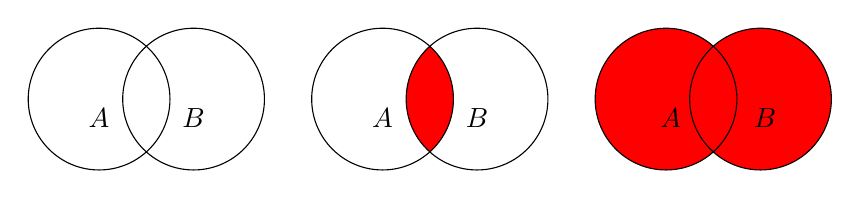
\begin{tikzpicture}[scale=0.6]

    \begin{scope}
      \clip (0,0) circle (1.5cm);
      \fill[red] (0:2) circle (1.5cm) ;
     \end{scope}

    \draw (-6,0) circle (1.5cm)  node [below] {$A$};
    \draw (-4,0) circle (1.5cm)  node [below] {$B$};

    \draw (0,0) circle (1.5cm)  node [below] {$A$};
    \draw (2,0) circle (1.5cm)  node [below] {$B$};

    \fill[red] (6,0) circle (1.5cm)  node [below] {$\black A$};
    \fill[red] (8,0) circle (1.5cm)  node [below] {$\black B$};
    \draw (6,0) circle (1.5cm) ; \draw (8,0) circle (1.5cm);

\end{tikzpicture}
\end{figure}
or \pause
\begin{align*}
A=\{1,2,3,4\}\qquad & A\cup B=\{1,2,3,4,5,6\}& A\cap B=\{3,4\}\\
B=\{3,4,5,6\}\qquad& &
\end{align*}
\end{frame}

\begin{frame}{Difference and symmetric difference}
\bl[$A-B$]{
The \textbf{set difference} $A-B$ of two sets $A$ and $B$ is the set of all elements of $A$ that are not in $B$}
\bl[$A\Delta B$]{
The \textbf{symmetric difference} of $A$ and $B$ is the set of all elements in $A$ but not $B$ or in $B$ but not $A$.
}

\begin{figure}
\center
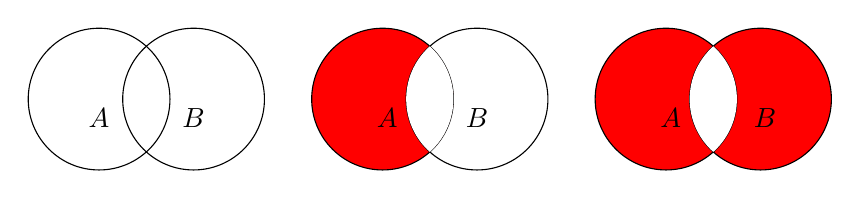
\begin{tikzpicture}[scale=0.6]

    
    \draw (-6,0) circle (1.5cm)  node [below] {$A$};
    \draw (-4,0) circle (1.5cm)  node [below] {$B$};

    \fill[red] (0,0) circle (1.5cm)  node [below] {$\black A$};
    \draw (0,0) circle (1.5cm);
    \draw (2,0) circle (1.5cm)  node [below] {$B$};

    \fill[red] (6,0) circle (1.5cm)  node [below] {$\black A$};
    \fill[red] (8,0) circle (1.5cm)  node [below] {$\black B$};
    \draw (6,0) circle (1.5cm) ; \draw (8,0) circle (1.5cm);

      \begin{scope}
      \clip (0,0) circle (1.5cm);
      \fill[white] (0:2) circle (1.5cm) ;
     \end{scope}

     \begin{scope}
      \clip (6,0) circle (1.5cm);
      \clip (8,0) circle (1.5cm);
      \fill[white] (7,0) circle (1.5cm) ;
     \end{scope}

\end{tikzpicture}
\end{figure}

or \pause
\begin{align*}
A=\{1,2,3,4\}\qquad & A- B=\{1,2\}& A\Delta B=\{1,2,5,6\}\\
B=\{3,4,5,6\}\qquad&B-A=\{5,6\} &
\end{align*}

\end{frame}



\begin{frame}{More formal definitions}
These operations can be formulated in terms of Boolean operators:
\begin{itemize}
\item $A\cup B=\{x: (x\in A)\vee (x\in B)\}$\pause
\item $A\cap B=\{x: (x\in A)\wedge (x\in B)\}$\pause
\item $A-B=\{x: (x\in A)\wedge (x\notin B)\}$\pause
\item $A\Delta B=(A-B)\cup (B-A)$
\end{itemize}
\end{frame}

\begin{frame}{Cartesian products}
\bl[$A\times B$]{
The \textbf{Cartesian product} of $A$ and $B$ is the set of all orered pairs (two-element lists) formed by taking an element of $A$ together with an element of $B$ in all possible ways. That is
\[
A\times B=\{(a,b): a\in A, b\in B\}
\]}
\[
A=\{1,2,3\},\qquad B=\{3,4,5\}
\]
\[
A\times B=\{(1,3), (1,4),(1,5),(2,3),(2,4),(2,5),(3,3),(3,4),(3,5)\}
\]
\[
B\times A=\{(3,1),(3,2),(3,3),(4,1),(4,2),(4,3),(5,1),(5,2),(5,3)\}
\]\vspace{-0.5cm}\pause

\center{\alert{In general $A\times B\neq B\times A$, but}}
\bl[Proposition]{
Let $A$ and $B$ be finite sets. Then $|A\times B|=|B\times A|=|A|\cdot|B|$.}

\end{frame}

\begin{frame}{Properties of set operations}
\begin{theorem}
Let $A$, $B$, and $C$ denote sets.
\begin{itemize}
\item Commutative properties:
\[
A\cup B=B\cup A,\qquad A\cap B=B\cap A
\] 
\item Associative properties:
\[
A\cup(B\cup C)=(A\cup B)\cup C,\qquad A\cap(B\cap C)=(A\cap B)\cap C
\]
\item Distributive properties:
\[
A\cup(B\cap C)=(A\cup B)\cap (A\cup C),\qquad A\cap(B\cup C)=(A\cap B)\cup (A\cap C)
\]
\item $A\cup \emptyset=A$ and $A\cap\emptyset=\emptyset$.
\end{itemize}
\end{theorem}
\end{frame}



\begin{frame}{Associativity for unions}

\begin{theorem}
Let $A$, $B$, and $C$ denote sets. Then
\[
A\cup(B\cup C)=(A\cup B)\cup C.
\]
\end{theorem}
We use Boolean identities 
\begin{proof}
\begin{align*}
A\cup(B\cup C)&=\{x:(x\in A)\vee(x\in B\cup C)\}=\\
&=\{x: (x\in A)\vee((x\in B)\vee(x\in C))\}=\\
&=\{x:((x\in A)\vee(x\in B))\vee(x\in C)\}=\\
&=\{x: (x\in A\cup B)\vee(x\in C)\}=\\
&=(A\cup B)\cup C\qedhere
\end{align*}\vspace{-0.5cm}
\end{proof}
\end{frame}

\begin{frame}{Alternative representation for the symmetric difference}
\begin{theorem}
Let $A$ and $B$ sets. Then
\[
A\Delta B=(A\cup B)-(A\cap B).
\]
\end{theorem}

\begin{figure}

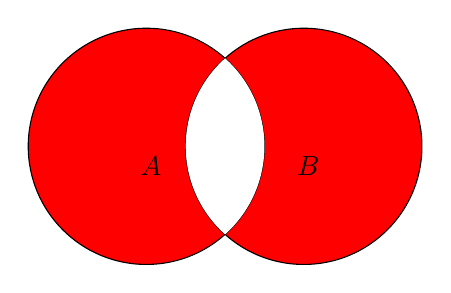
\begin{tikzpicture}
    \fill[red] (0,0) circle (1.5cm)  node [below] {$\black A$};
    \fill[red] (2,0) circle (1.5cm)  node [below] {$\black B$};
    \draw (0,0) circle (1.5cm) ; \draw (2,0) circle (1.5cm);


     \begin{scope}
      \clip (0,0) circle (1.5cm);
      \clip (2,0) circle (1.5cm);
      \fill[white] (1,0) circle (1.5cm) ;
     \end{scope}

\end{tikzpicture}
\end{figure}

\end{frame}

\begin{frame}
\begin{proof}
Let $A$ and $B$ be sets.

\enumb
\item[(1)] Suppose $x\in A\Delta B$.\only<2>{\color{blue}}\uncover<2->{ Thus $x\in (A-B)\cup (B-A)$. This means either $x\in A-B$ or $B-A$.}
\itemb
\item \only<2>{\color{blue}}\only<3->{\color{black}}\uncover<2->{ Suppose $x\in A-B$.}\only<3>{\color{blue}}\uncover<3->{ So $x\in A$ and $x\notin B$.} \only<4>{\color{blue}}\uncover<4->{ Since $x\in A$, we have $x\in A\cup B$. Since $x\notin B$, we have $x\notin A\cap B$.}\only<5>{\color{blue}}\uncover<5->{ Therefore $x\in (A\cup B)-(A\cap B)$.} 
\item \only<2>{\color{blue}}\only<3->{\color{black}}\uncover<2->{ Suppose $x\in B-A$.}\only<6>{\color{blue}}\uncover<6->{ Then $x\in (A\cup B)-(A\cap B)$ similarly.}
\iteme
\color{black}Therefore $x\in (A\cup B)-(A\cap B)$.

\item[(2)]\color{black} Suppose $x\in (A\cup B)-(A\cap B)$.\only<8>{\color{blue}}\uncover<8->{ Thus $x\in A\cup B$ and $x\notin A\cap B$.}\only<9>{\color{blue}}\uncover<9->{ This means that $x$ is in $A$ or $B$ but not both. Thus either $x\in A-B$ or $x\in B-A$.}\only<10>{\color{blue}}\uncover<10->{ So $x\in (A-B)\cup(B-A)$. Therefore $x\in A\Delta B$.}

\color{black}~~~~Therefore $A\Delta B=(A\cup B)-(A\cap B)$.\qedhere
\enume
\end{proof}
\end{frame}

\section{Combinatorial proofs}

\begin{frame}{The size of a union}
\bl[Proposition (Inclusion-Exclusion formula)]{
Let $A$ and $B$ be finite sets. Then $|A|+|B|=|A\cup B|+|A\cap B|$.}\pause

\begin{proof}
Assign label $'A'$ to the objects in $A$ and label $'B'$ to objects in $B$. 

~~~~On one hand we clearly handed out $|A|+|B|$ labels. 

~~~~On the other hand, there are $|A\cup B|$ objects that got at least a label and exactly $|A\cap B|$ elements got doubly labeled. Therefore $|A\cup B|+|A\cap B|$ counts all elements that receive a label, double counting the ones that have two labels. Therefore the total number of labels also equals this number.

~~~~ Since $|A+B|$ and $|A\cup B|+|A\cap B|$ give the answer to the same question, they must be equal.\qedhere
\end{proof}
\end{frame}

\begin{frame}{Inclusion-exclusion formula for two sets}
\bl[]{\center{$|A\cup B|=|A|+|B|-|A\cap B|$}}

For example: How many integers in the range $1$ to $1000$ (inclusive) are divisible by $2$ or by $5$?\pause
\[
A=\{x\in\mathbb{Z}: 1\leq x\leq 1000\textrm{ and }2|x\}
\]
\[
B=\{x\in\mathbb{Z}: 1\leq x\leq 1000\textrm{ and }5|x\}
\]\pause
Then $|A|=500$ and $|B|=200$. Also note
\[
A\cap B=\{x\in\mathbb{Z}: 1\leq x\leq 1000\textrm{ and }10|x\}
\]
and therefore $|A\cap B|=100$.\pause Therefore
\[
|A\cup B|=|A|+|B|-|A\cap B|=500+200-100=600.
\]\pause
Therefore there are $600$ integers in the range $1$ to $1000$ that are divisible by either $2$ or $5$.
\end{frame}

\begin{frame}{A combinatorial proof}
\bl[]{To prove an equation of the form LHS=RHS:\\
~~~~Pose a question of the form, 'In how many ways...?'\\
~~~~~~~~On one hand argue why LHS is the correct answer.\\
~~~~~~~~On the other hand argue why RHS is the correct answer.\\
~~~~Therefore LHS=RHS}
\end{frame}

\begin{frame}{Disjoint sets}
\bl[Definition]{
We call the sets $A$ and $B$ \textbf{disjoint} if $A\cap B=\emptyset$.}\pause
In this case the inclusion exclusion formula reads:
\bl[Addition principle]{Let $A$ and $B$ finite sets. If $A$ and $B$ are disjoint, then 
\[
|A\cup B|=|A|+|B|
\]}\pause
\center{\alert{What about two or more sets?}}
\end{frame}

\begin{frame}{Disjoint, pairwise disjoint sets}

\bl[Definition]{
The sets $A_1, A_2,\dots A_n$ are \textbf{pairwise disjoint} provided $A_i\cap A_j=\emptyset$ whenever $i\neq j$.}\pause

For example, $A=\{1,2,3\}$, $B=\{4,5,6\}$ and $C=\{7,8,9\}$ are pairwise disjoint.\pause

\bl[Extended addition principle]{
If the sets $A_1,A_2,\dots,A_n$ are pairwise disjoint sets, then
\[
|A_1\cup A_2\cup\dots\cup A_n|=|A_1|+|A_2|+\dots+|A_n|
\]}\pause
In a more compact notation:
\[
\left|\cup_{k=1}^nA_k\right|=\sum_{k=1}^n|A_k|
\]
\end{frame}

\begin{frame}{Disjoint, pairwise disjoint sets}
\bl[Definition]{
The sets $A_1, A_2,\dots A_n$ are \textbf{pairwise disjoint} provided $A_i\cap A_j=\emptyset$ whenever $i\neq j$.}

Note that this is stronger than requiring
\[
A_1\cup...\cup A_n=\emptyset.
\]

Consider for example
\[
A_1=\{1,2\}, \qquad A_2=\{2,3\}, \qquad A_3=\{3,4\}.
\]
Then
\[
A_1\cap A_2=\{2\}\neq \emptyset,\qquad A_1\cup A_2\cup A_3=\emptyset.
\]
\end{frame}

\begin{frame}{Problem 7 from Worksheet 5}
\vspace{-0.2cm}

\bl[Proposition]{\vspace{-0.1cm}
\[
2^0+2^1+\dots 2^{n-1}=2^n-1
\]}

\underline{Let $A=\{x\in 2^{\{1,\dots, n\}}: x\neq\emptyset\}$. What is $|A|$?}
\vspace{0.1cm}
\itemb
\item Easy answer: $|A|=2^n-1$.
\item On the other hand, let
\[
A_j=\{x\in 2^{\{1,\dots, n\}}: \textrm{largest element in $x$ is $j$}\}
\]\vspace{-0.5cm}

\itemb
\item A subset cannot have two largest elements $\to$ $A_j\cap A_i=\emptyset$.
\item Every nonempty set has a largest element $\to$ $A=\cup_{j=1}^nA_j$.
\item $|A_j|=2^{j-1}$ because $j$ is in every $x\in A_j$ and $x$ can be completed by any subset of $\{1,\dots,j-1\}$.
\iteme
By the extended addition principle:
\[
|A|=|A_1|+\dots+|A_n|=2^0+\dots 2^{n-1}
\]
\iteme 
Since both the left and the right hand side answer the same question, they must be equal.
\end{frame}
\end{document}